%----------------------------------------
\begin{frame}
  \frametitle{Zones: time is cut at task boundaries} \small

{\centering
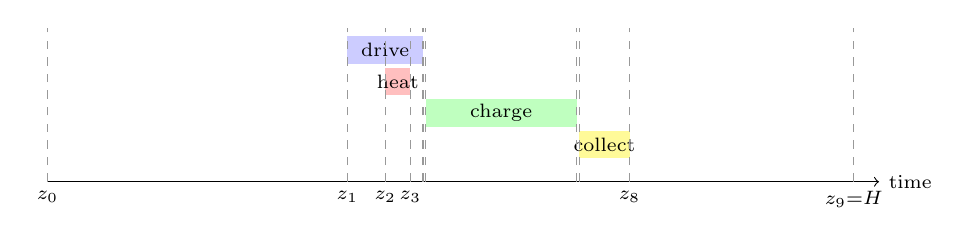
\begin{tikzpicture}[x=0.032cm, y=0.5cm, font=\scriptsize]
  % tasks
  \fill[blue!20]   (119,3) rectangle (149,3.7); \node at (134,3.35) {drive};
  \fill[red!25]    (134,2.2) rectangle (144,2.9); \node at (139,2.55) {heat};
  \fill[green!25]  (150,1.4) rectangle (210,2.1); \node at (180,1.75) {charge};
  \fill[yellow!40] (211,0.6) rectangle (231,1.3); \node at (221,0.95) {collect};
  % axis
  \draw[->] (0,0) -- (330,0) node[right] {time};
  \foreach \z/\l in {0/z_0,119/z_1,134/z_2,144/z_3,149/,150/,210/,211/,231/z_8}
    { \draw[dashed, black!40] (\z,0) -- (\z,3.9); \node[below] at (\z,0) {$\l$}; }
  \node[below] at (320,0) {$z_9{=}H$};
  \draw[dashed, black!40] (320,0) -- (320,3.9);
\end{tikzpicture}\par}

\vspace{0.3cm}
\begin{itemize}
\item Zone boundaries $z_0 < z_1 < \dots$ are SMT variables; every task start and end
      {\bf is} a zone boundary, and vice versa. Nothing changes inside a zone.
\item Each timeline gets {\bf one value per zone}, so the formula is $O(\#\mathit{tasks} \times \#\mathit{timelines})$,
      independent of the horizon.
\item Impacts are case splits on which boundary a task's start or end equals.
\end{itemize}

\end{frame}

%----------------------------------------
\begin{frame}
  \frametitle{The one nonlinear term} \small

A rate timeline $\ell$ has a value $v[j]$ and a rate $\rho[j]$ per zone:

\[
v[j{+}1] \;=\; \mathit{clamp}\big(\,v[j] \;+\; \underbrace{\rho[j] \cdot (z_{j+1} - z_j)}_{\text{rate} \,\times\, \text{zone width}} \;+\; \Delta[j]\,\big)
\]

\vspace{0.2cm}
Both factors are unknowns: the only product of two variables in the encoding.

\pause
\vspace{0.4cm}
\begin{itemize}
\item It is what makes batteries hard. A network where many tasks drain one battery
      couples them all through these products.
\item It is also an opportunity: {\bf fix the times, and the formula becomes linear}.
      Realizability exploits exactly this.
\end{itemize}

\end{frame}

%----------------------------------------
\begin{frame}
  \frametitle{Checking a property} \small

Temporal formulas are unfolded over the zones, e.g.
\[
\mathtt{always}\ \varphi \;=\; \bigwedge_j \varphi[j]
\qquad
\mathtt{eventually}\ \varphi \;=\; \bigvee_j \varphi[j]
\]

\vspace{0.2cm}
To prove $\varphi$ for {\em all} schedules, ask \zthree{} for a schedule violating it:

\[
\exists i\, \exists s\, .\ \mathit{valid}(i,s) \wedge \neg\varphi(s)
\]

\vspace{0.2cm}
\begin{itemize}
\item UNSAT: $\varphi$ \holds{}, for every schedule.
\item SAT: \violated{}, and the model is the counterexample schedule.
\end{itemize}

\vspace{0.2cm}
Same idea for {\tt final \{ ... \}}: the state at the end of every schedule.

\end{frame}
